\chapter{Auswahl elektronischer Komponenten und Verschaltung}\label{ch:komp}
\section{Anforderungen an die Komponenten}
Die benötigten elektronischen Komponenten werden üblicherweise in \glqq Passive Bauelemente\grqq{} und \glqq Aktive Bauelemente\grqq{} untergliedert. Unter passiven Bauelementen versteht man Komponenten, die das Eingangssignal ohne Verstärkung übertragen. Aktive Bauelemente benötigen meist eine Hilfsquelle und können somit ein Eingangssignal verstärken \cite[S. 25]{haendschke}. Für den Einsatz elektronischer Komponenten im Automobilbereich hat sich für passive Bauteile die Zertifizierung nach AEC-Q200 und für aktive Bauteile nach AEC-Q100 als Qualitätsstandard etabliert. Anhand dieser Zertifizierungen wird eine nachweisliche Belastbarkeit der Bauelemente nach dem jeweiligen Standard definiert. Für die Anforderungen an die Platine werden die passiven Bauelemente nach AEC-Q200 und die aktiven Bauelemente nach AEC-Q100 mindestens in Grade 2 eingestuft, um den Temperaturanforderung bis \SI{105}{^\circ C} gerecht zu werden\cite[S.6]{aecq}. 
\subsection{Passive Bauteile}
Unter die benötigten passiven Bauteile fallen lediglich Kondensatoren und Widerstände, welche nach dem AEC-Q200 Standard ausgewählt werden. Anforderung ist danach eine hohe thermische Belastbarkeit von mindestens \SI{105}{^\circ C}. Um eine geringe Bauteilgröße für die Platine zu bekommen sollten sowohl Widerstände als auch Kondensatoren als SMD (\textit{surface-mounted device}) gekauft werden. Für Entkopplungskondensatoren werden nach \cite[S.7]{ldo} Keramikkondensatoren mit XR7 präferiert. Als Baugröße bei manueller Bestückung bieten sich die Standardgrößen 1206 oder 0805 (Angabe in $\frac{1}{100}$ Zoll), welche noch per Hand lötbar sind. Die Widerstände für die Sensorik müssen mit sehr hoher Präzision gewählt werden um Messfehler aufgrund falscher Widerstandswerte zu vermeiden. Im Anwendungsfall bieten sich daher Dünnschichtwiderstände an.
\subsection{Aktive Bauteile}
Die aktiven Bauelemente der Platine müssen dafür ausgelegt werden, um im späteren alle Anforderungen aus der Anforderungsliste gerecht zu werden. Demnach müssen sie in ihrer logischen Verschaltung einerseits in der Lage sein den Tauchspulenaktor anzusteuern und auszuregeln, andererseits aber auch die Bedingungen über Leistungsaufnahme etc. erfüllen. Kern der Platine ist ein Mikrocontroller, welcher schnell genug sein muss um Gangwechsel in weniger als 0,1s durchzuführen. Weiterhin muss der Mikrocontroller die CAN-Kommunikation mit der MicroAutobox unterstützen. Da der Mikrocontroller nicht über die \SI{13,8}{V} der Autobatterie gespeist werden kann, wird ein Spannungsregler benötigt, welcher auf die Betriebsspannung des Mikrocontrollers regelt. Um aus den physikalischen Bussignalen CAN-HIGH und CAN-LOW für den Mikrocontroller verwertbare Signale zu erhalten wird ein CAN-Transciever benötigt. Über ihn ist eine Kommunikation des Mikrocontrollers mit der CAN-Peripherie erst möglich. Zum Regeln des Tauchspulenaktors ist ein Motortreiber nötig, welcher vom Mikrocontroller angesteuert wird um die Spannung an den Tauchspulenaktor durchzuschalten. Eine Ansteuerung des Motortreibers mittels PWM-Signal sollte möglich sein. Der Motortreiber muss dabei für zukünftige Aktorkonfigurationen für Ströme bis zu 55A ausgelegt sein. Des Weiteren wird eine Spannungsebene von \SI{5}{V} benötigt um die Lagesensorik des Aktors zu unterstützen, wofür ein zweiter Spannungsregler eingeplant werden muss.
\begin{figure}[H]%
\centering
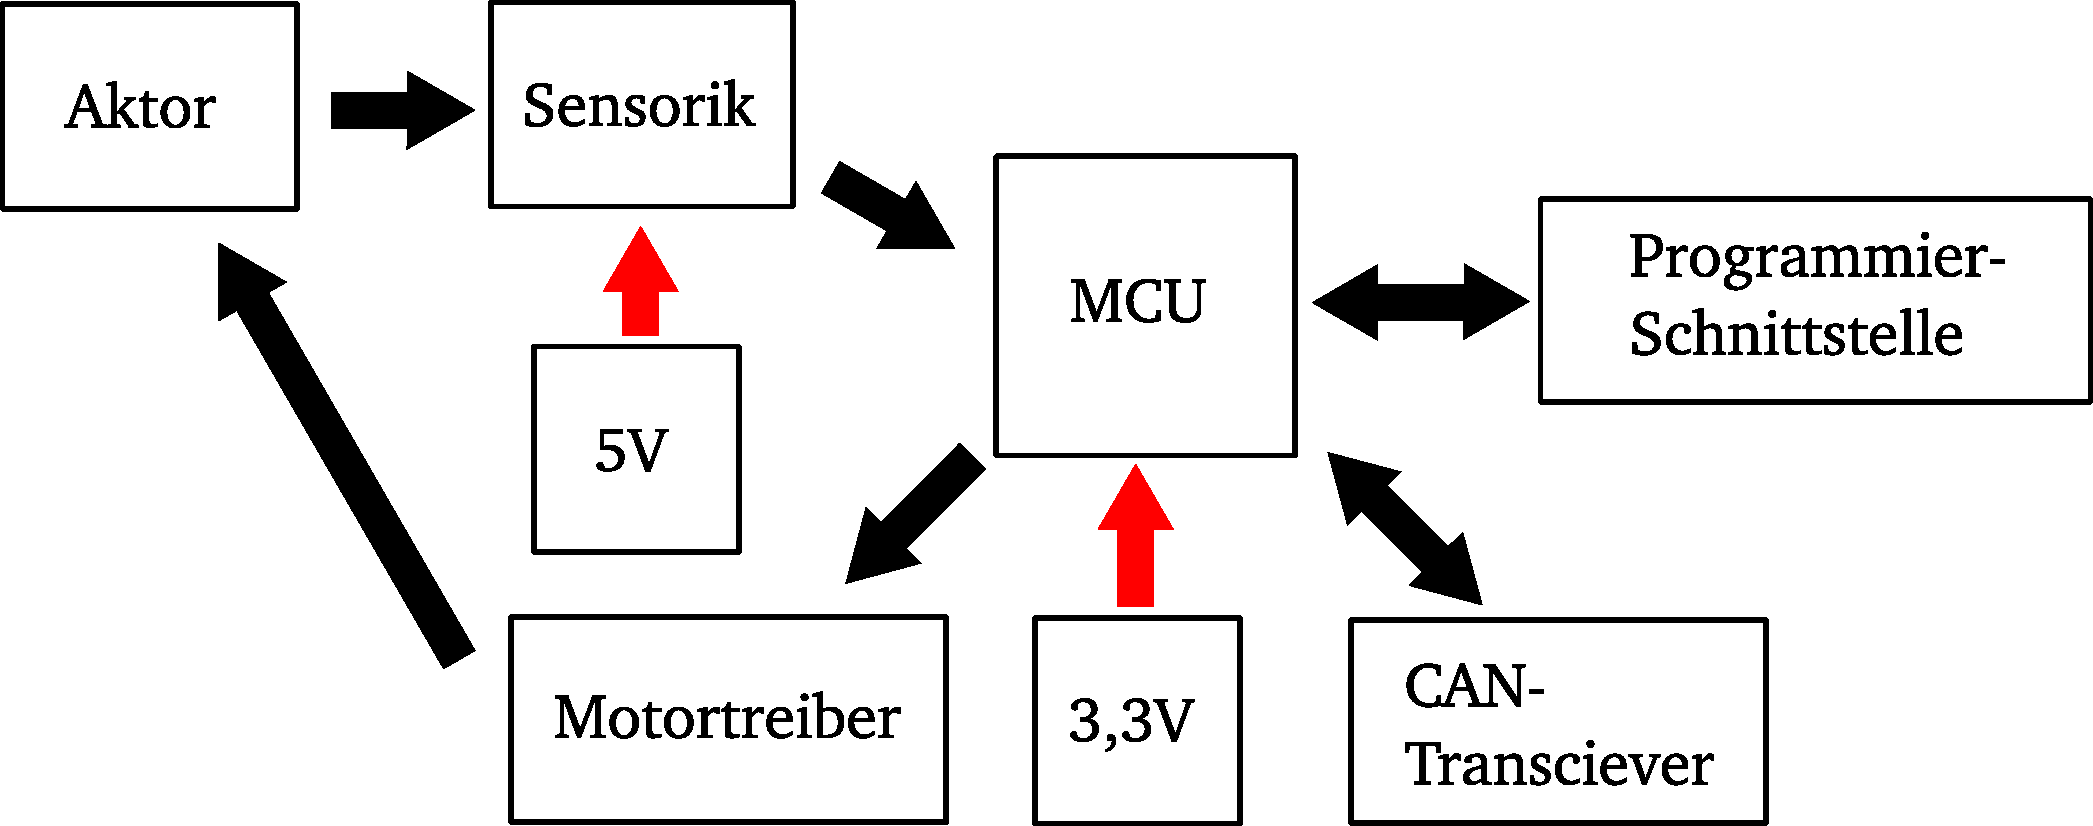
\includegraphics[width=300pt]{./Bilder/anf.pdf}%
\caption{Aktive Bauelemente}%
\label{fig:anf}%
\end{figure}
\section{Komponentenauswahl}
Anhand der Anforderungen an die Platinenelemente sind die endgültigen Komponenten der Platine zu wählen. Es müssen Mikrocontroller, Spannungsregler, CAN-Transciever und Motortreiber ausgewählt werden. Weiterhin wird eine Temperaturbeständigkeit bis \SI{105}{^\circ C} gefordert.
\subsection{Mikrocontroller}
Die Recheneinheit zur Regelung des Tauchspulenaktors ist ein STM32F405RGT7. Dieser ist mit verschiedenen Pin-Anzahlen erhältlich und auf der Platine aus Platzgründen in der Ausführung LQFP64 mit 64 Pins verbaut. Der Mikrocontroller zeichnet sich durch seine hohe CPU-Geschwindigkeit von \SI{168}{MHz} und seine große Programm-Speichergröße von \SI{1}{MB} aus. Die Produktbezeichnung \glqq T7\grqq{} steht dabei für die zulässige Betriebstemperatur von -40...\SI{105}{^\circ C}. Weiterhin besitzt dieser Mikrocontroller die geforderten CAN-Schnittstellen, anhand derer mit der MicroAutobox kommuniziert werden soll. In \autoref{fig:mcumin} ist die Minimalbeschaltung des Mikrocontrollers zu sehen. Diese ist dem Datenblatt des STM32 entnommen\cite[S.77]{stm32}. Die Pins mit den Bezeichnungen VDD...VDD\_4 sind die Versorgungspins des Mikrocontrollers. An diesen Pins liegt die Versorgungsspannung an, welche nach dem Datenblatt zwischen 1,8 und \SI{3,6}{V} liegt. Diese ist aufgrund der Versorgungsspannung anderer Bauteile zu VDD = \SI{3,3}{V} gewählt. Die VDD Pins werden durch die Keramikkondensatoren C7-C11 entkoppelt, welche nach dem Datenblatt dimensioniert sind und möglichst nah an den dem jeweiligen VDD-Pin plaziert werden sollen. Die Entkopplung wird benötigt um Welligkeiten der Spannungsversorgung zu filtern und parasitäre Induktivitäten zu entkoppeln\cite{decoupling}. Der Pin VBAT wird unter Anderem für die Versorgung der Echtzeituhr (\textit{RTC}), der Backup-Register und des Backup-SRAMs genutzt und wird, wenn keine zweite Spannungsversorgung neben der Hauptversorgung vorhanden ist, ebenfalls an VDD angeschlossen \cite[S.31]{stm32}. VDDA ist der Pin für die Spannungsversorgung des Analog-Digital-Converters (\textit{ADC}) und wird ebenfalls mit der Versorgungsspannung von VDD angeschlossen. Die Kapazitäten C5 und C6 sind nach den Herstellerangaben dimensioniert und sorgen ebenfalls für eine Entkopplung der Spannungsversorgung. Die Induktivität L1 bietet die Möglichkeit, je nach Welligkeit der Versorgungsspannung, diese über einen LC-Filter zu filtern um eine bessere Auflösung des ADCs zu gewährleisten. Wenn dieser Filter nicht benötigt wird, sollte L1 durch einen \SI{0}{\Omega} Widerstand ersetzt werden.
VCAP\_1 und VCAP\_2 sind die Ausgänge des internen Voltage Regulators des STM32 und C5 bzw. C6 werden zur Glättung der intern geregelten Spannung genutzt\cite[S.77]{stm32}. Die Pins VSS, VSS\_2, VSSA sind die GND Anschlüsse für den Mikrocontroller und den internen ADC.
\begin{figure}[H]%
\centering
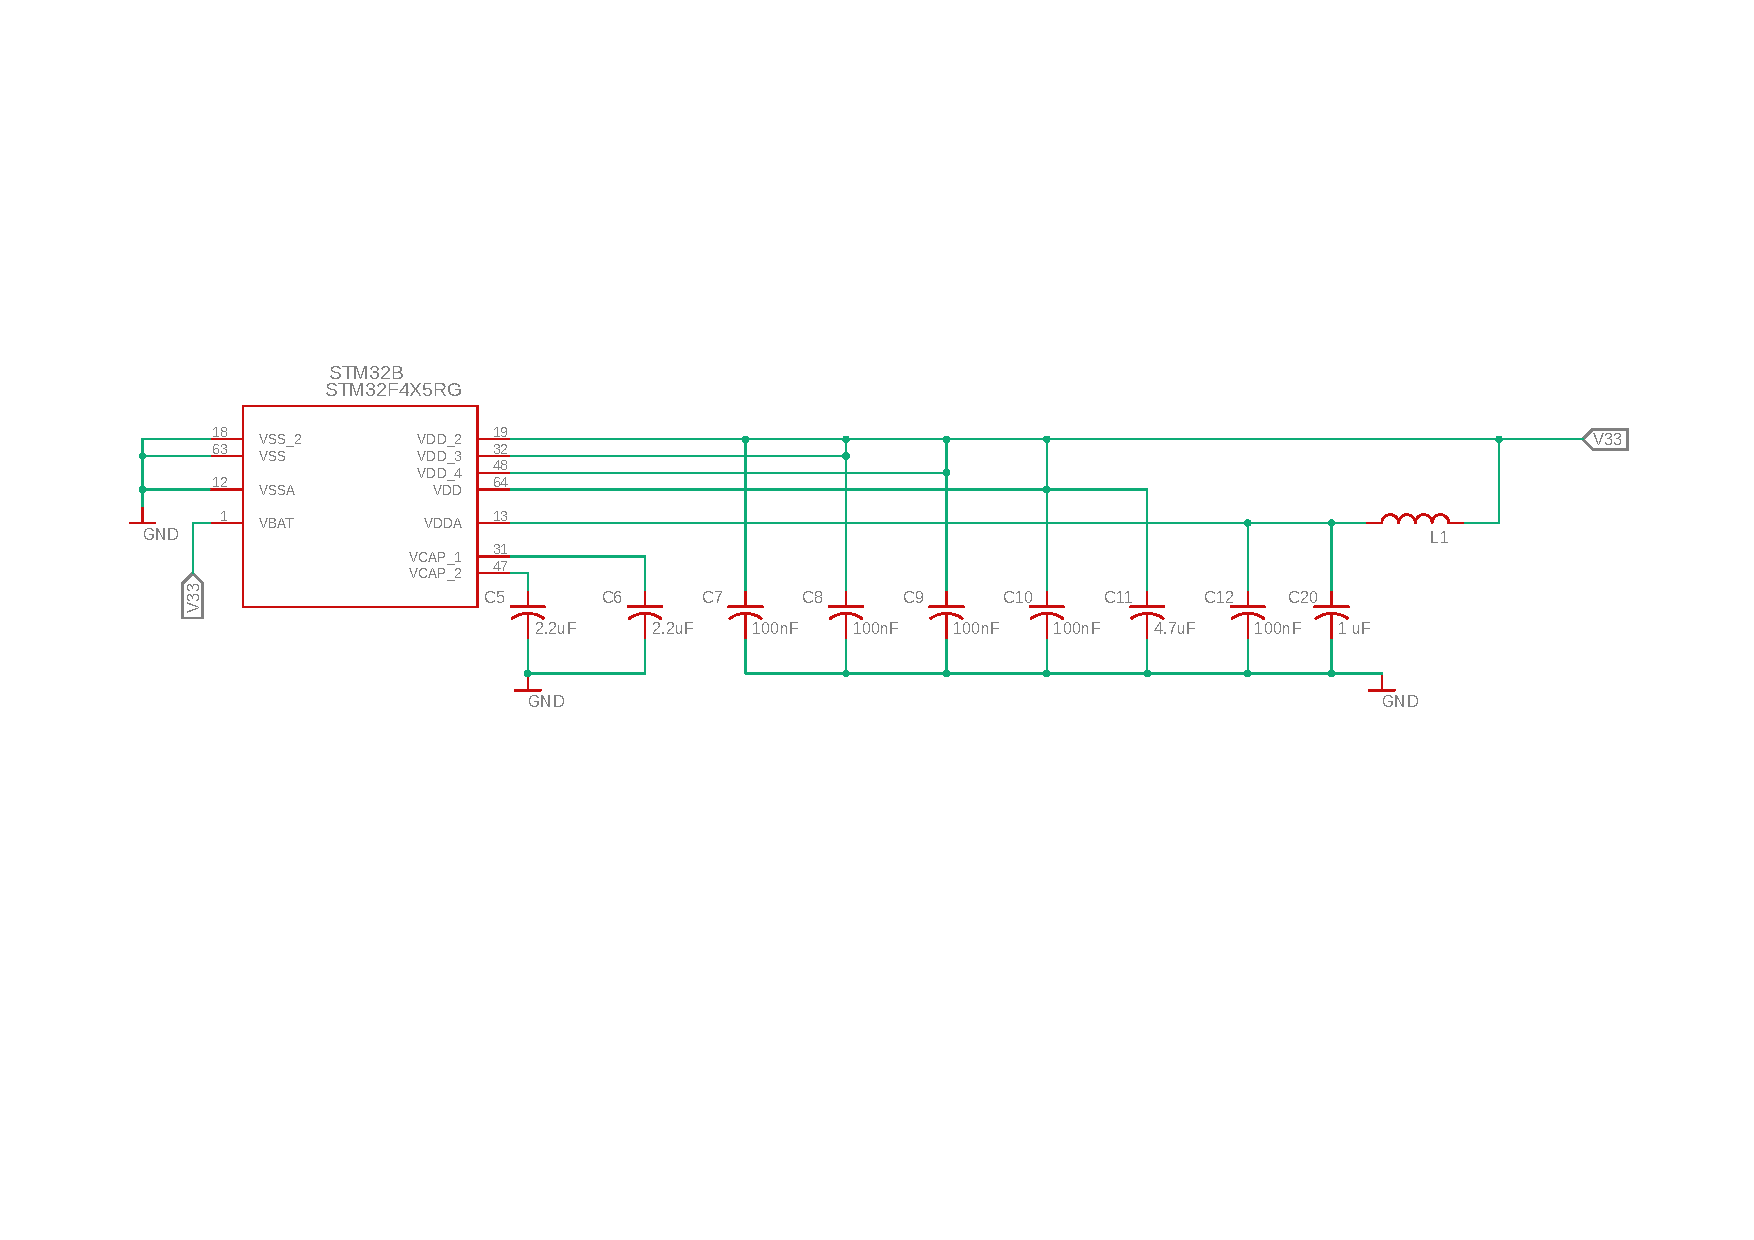
\includegraphics[width=\columnwidth]{./Bilder/MCU_MIN.pdf}%
\caption{Minimalbeschaltung des STM32F405RGT7}%
\label{fig:mcumin}%
\end{figure}

In \autoref{fig:mcupin} sind die Pin-Belegungen des Mikrocontrollers dargestellt, welche durch \autoref{tab:pins} genauer beschrieben sind. Unter Sensorik fallen die Ausgänge für Lagesensorik, Temperatursensorik und Messung der Versorgungsspannung. Die UART Pins können zum debuggen auf der endgültigen Platine genutzt werden. Zur CAN-Kommunikation werden die Pins CAN1-TX(PA11) und CAN1-RX(PA12) benötigt, womit der Mikrocontroller über einen CAN-Transciever Nachrichten an die MicroAutobox senden und empfangen kann. Zum Programmieren des Mikrocontrollers wird eine Serial Wire Debug (kurz: \textit{SWD}) Schnittstelle aufgebaut, welche sich mittels externem ST-Link/V2 mit dem Computer verbinden lässt. Dazu werden die jeweiligen Pins über den Platinenstecker nach außen geführt. Weiterhin müssen Pins zum Beschalten der H-Brücke und zum Auslesen der Strommessungen belegt werden. Die Pins OSC\_IN und OSC\_OUT sind zum Anschließen eines externen Quarzes, welcher als Taktgeber für den Mikrocontroller genutzt wird. Der Pin NRST wird für den Fall eines notwendigen Resets herausgeführt.

\noindent\begin{minipage}{0.75\textwidth}
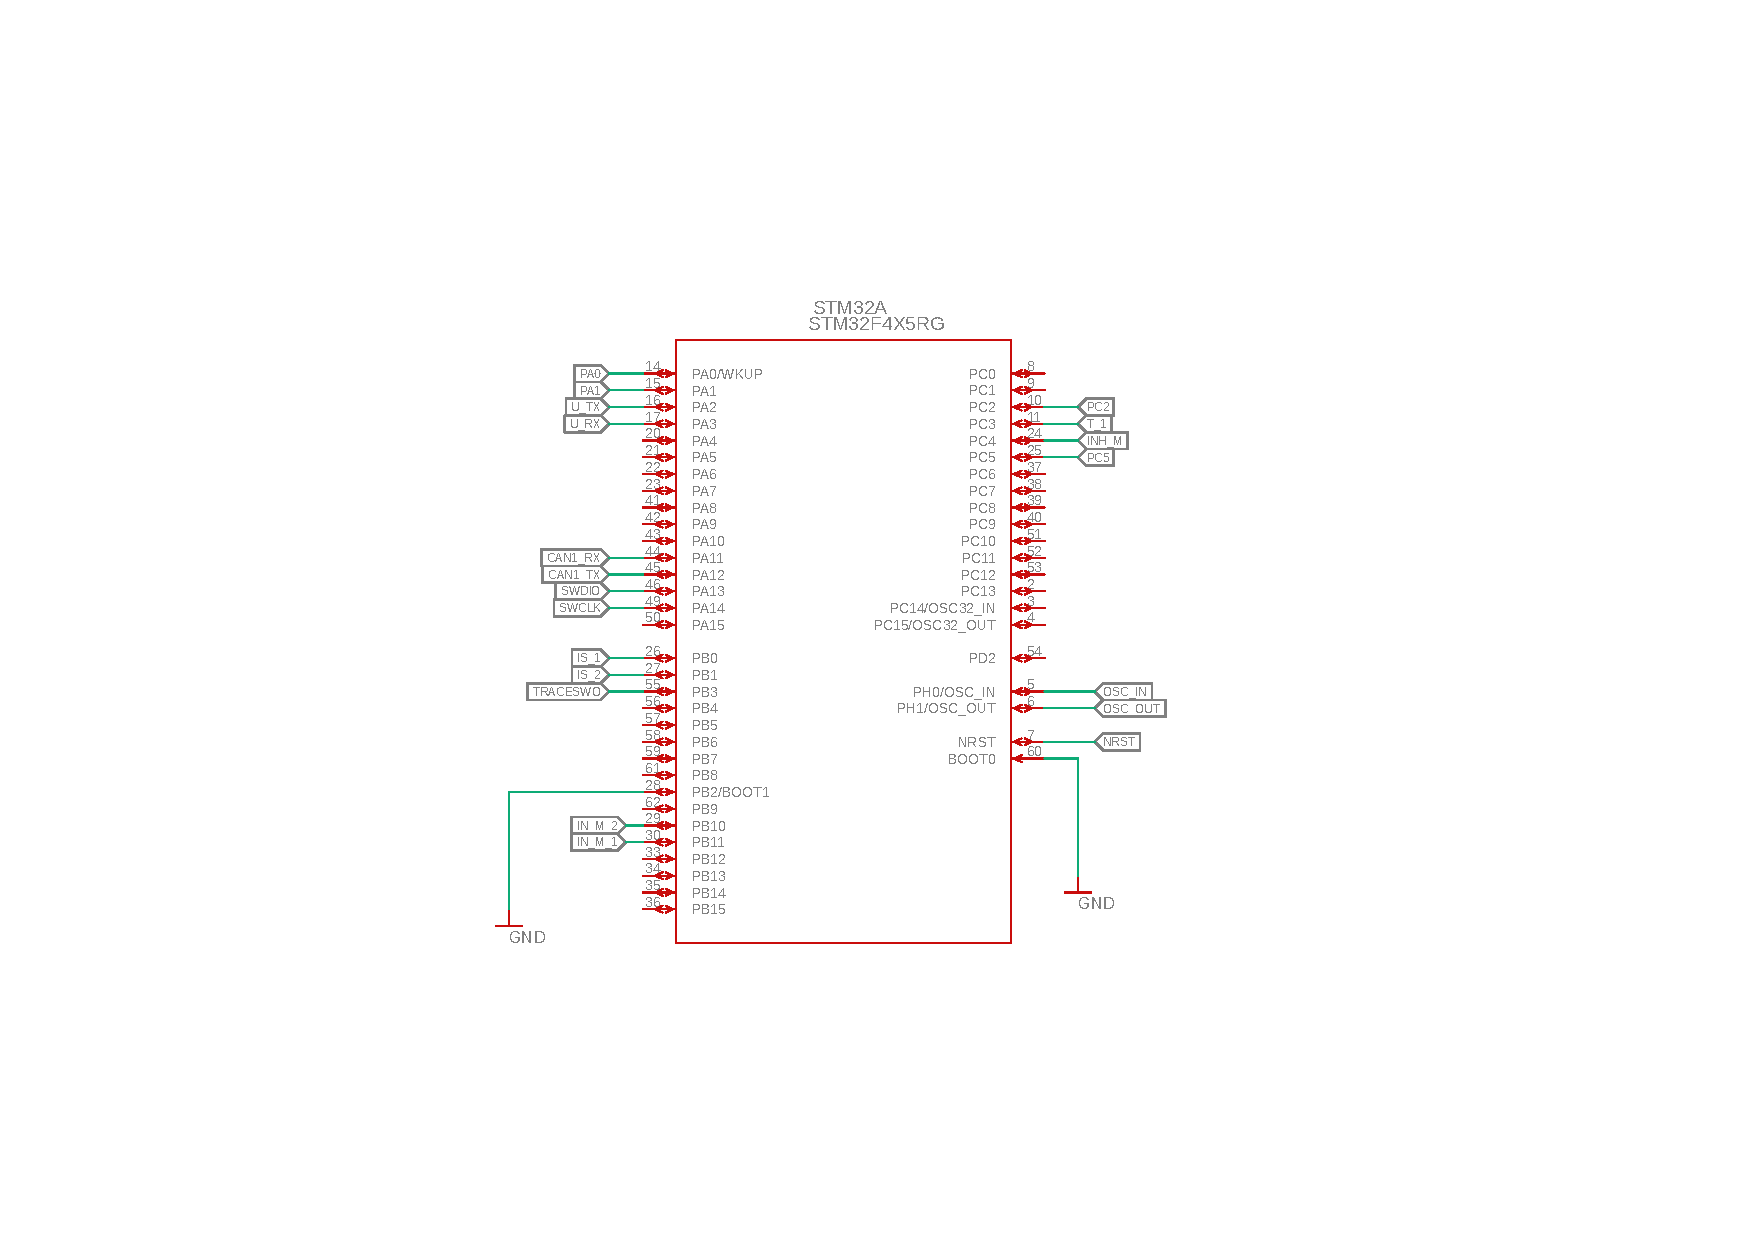
\includegraphics[width=\textwidth]{./Bilder/MCU_PINS.pdf}
\end{minipage}
\noindent\begin{minipage}{0.1\textwidth}
\begin{tabular}{l | l}
			Pin & Funktion\\ \hline
			PA0& Sensorik\\
			PA1& \\
			PB0&\\
			PB1&\\
			PC2&\\
			PC3&\\
			PC5&\\
			PA2&UART\\
			PA3&\\
			PA11&CAN\\
			PA12&\\
			PA13&SWD\\
			PA14&\\
			PB3&\\
			PB0 & H-Brücke\\
			PB1 &\\
			PB10&\\
			PB11&\\
			PC4&\\
			OSC\_IN&Quarz\\
			OSC\_OUT&\\
			NRST & Reset
		\end{tabular}
\end{minipage}

\noindent\begin{minipage}{0.75\textwidth}
\captionof{figure}{Pin-Belegung des Mikrocontrollers}
\label{fig:mcupin}
\end{minipage}
\noindent\begin{minipage}{0.2\textwidth}
	\captionof{table}{Pin-outs}
	\label{tab:pins}
\end{minipage}
\hspace{1cm}
\newline
\\
Wichtig bei der Beschaltung ist außerdem die Belegung von BOOT0 und BOOT1, welche den Speicherbereich definieren aus dem der Mikrocontroller beim Startvorgang sein Programm lädt. Nach \autoref{tab:boot} muss für den Start im Main Flash memory BOOT0 auf GND-Niveau gesetzt werden, während die Belegung von BOOT1 undefiniert ist und somit mit GND belegt werden kann.

\begin{table}[H]%
\centering
\begin{tabular}{c c c c}
BOOT1 & BOOT0 & Boot mode & Aliasing \\ \hline
x & 0 & Main Flash memory & Main Flash memory is selected as the boot space\\
0 & 1 & System memory & System memory is selected as the boot space\\
1 & 1 & Embedded SRAM & Embedded SRAM is selected as the boot space
\end{tabular}
\caption{Boot modes des STM32F405RGT7 nach \cite[S.69]{stmref}}
\label{tab:boot}
\end{table}

Um möglichst akurate Taktraten zu haben und somit Schaltvorgänge und Sensorikdaten genau und reproduzierbar zu machen, wird wie vom Hersteller des Mikrocontrollers empfohlen ein externer Taktgeber benutzt\cite[S.218]{stmref}. Auf der Platine wird hierbei ein ABLS-8.000MHZ-K4T von Abracon genutzt, welcher eine Nennfrequenz von 8MHz hat. \autoref{fig:quarz} zeigt die letztendliche Verschaltung auf der Platine. Die Lastkapazitäten CQ1 und CQ2 von \SI{22}{pF} sind dabei nach dem Datenblatt des Herstellers gewählt. Die Widerstände R19 und R20 sind einerseits verbaut, um den externen Quarz vom Mikrocontroller trennen zu können, andererseits wird R20 benutzt, um den Stromfluss des Quarzes zu beschränken \cite[S.16]{stmquarz}. Nach \cite[S.16]{stmquarz} lässt sich eine Abschätzung von R20 über
\begin{align*}
R_{20} = \frac{1}{2\pi f C_{Q1}}
\end{align*}
gewinnen. Damit ergibt für R20 sich ein Richtwert von etwa \SI{900}{\Omega} bei CQ1 = 22pF. Ein zu niedriger Widerstand erhöht die Verlustleistung über den Quarz, während ein höherer Widerstand zum Stillstand der Oszillation führen kann. Auf der Platine ist ein Widerstand von \SI{1}{k\Omega} gewählt.

\begin{figure}[H]%
\centering
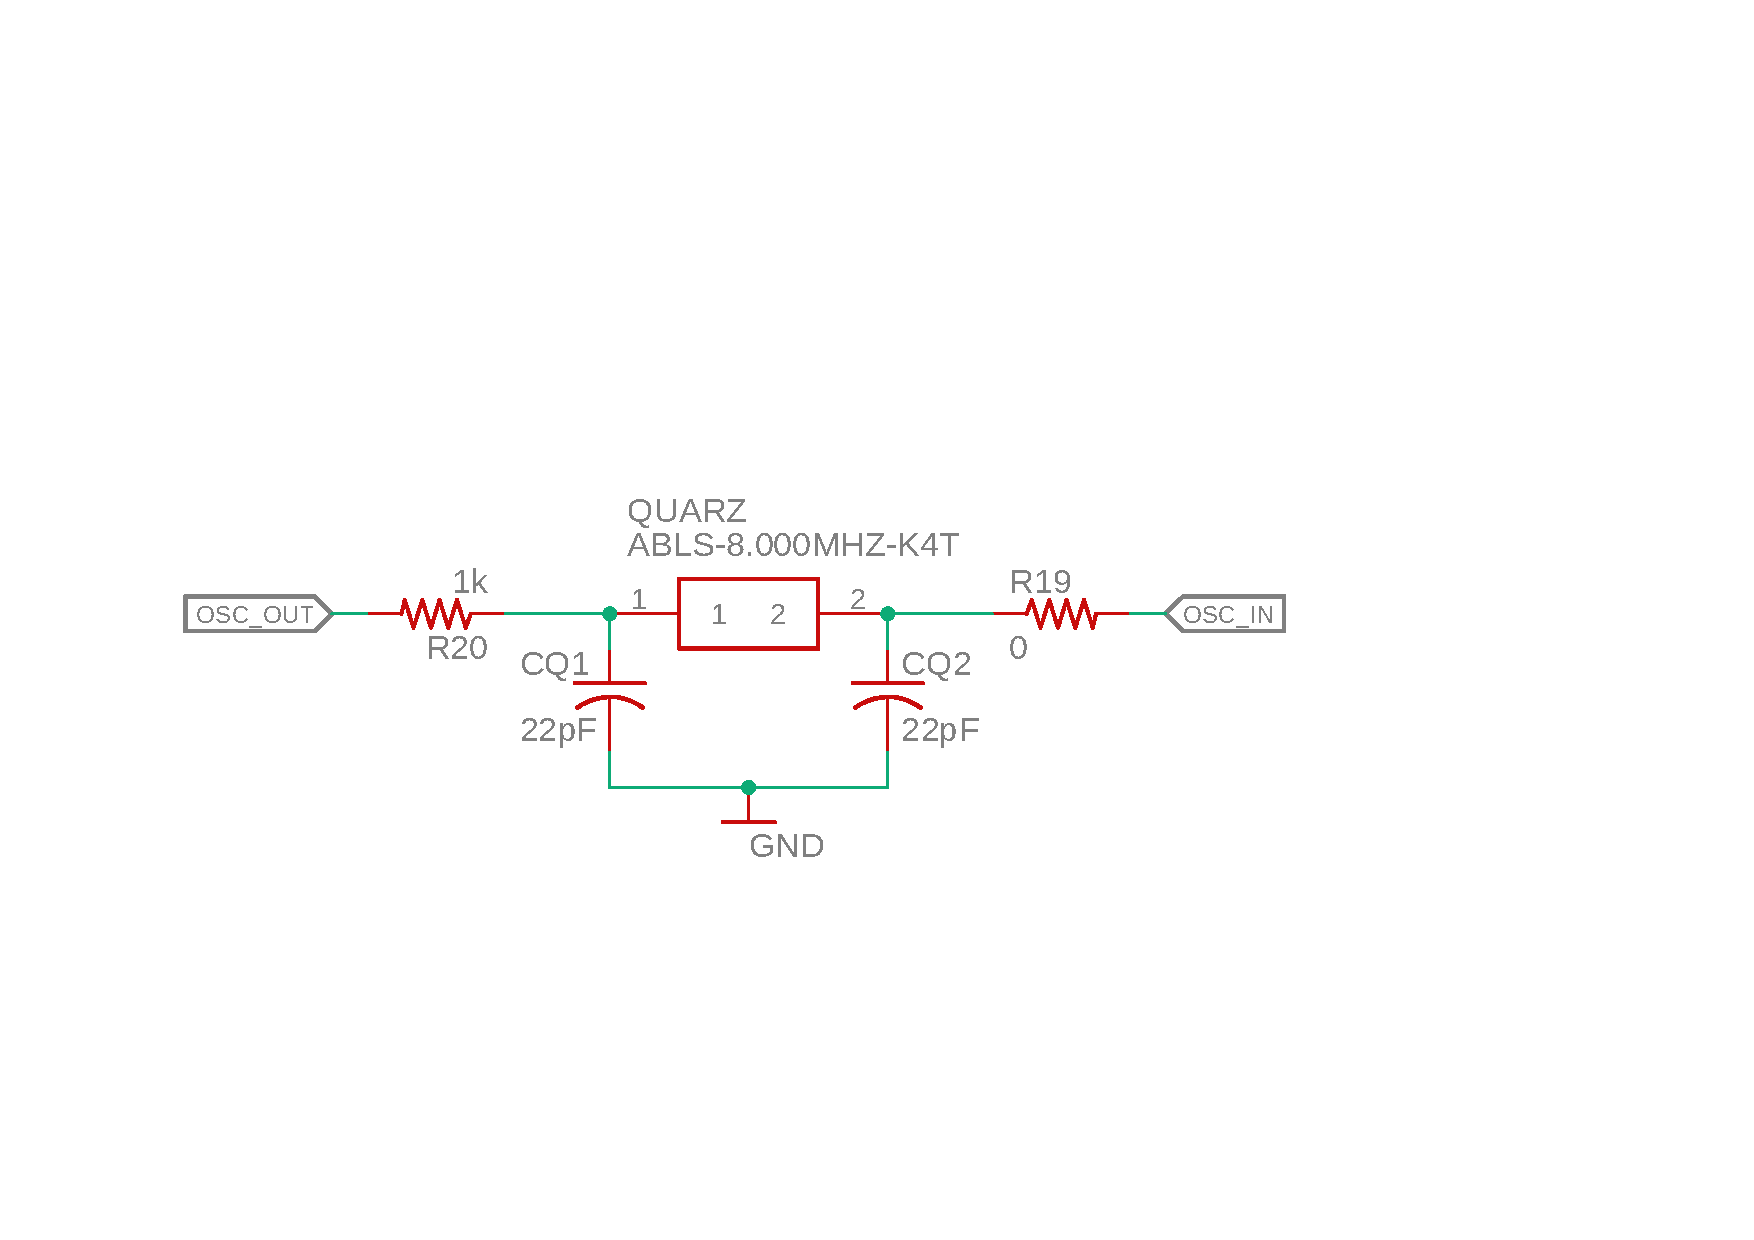
\includegraphics[width=300pt]{./Bilder/quarz.pdf}%
\caption{Anschluss externer Quarz}%
\label{fig:quarz}%
\end{figure}

\subsection{CAN-Transciever}
Zur Kommunikation des Mikrocontrollers mit der MicroAutobox ist eine Signalübertragung über CAN vorgesehen. Da der Mikrocontroller die physikalischen Bussignale nicht verarbeiten kann, wird die Kommunikation des Mikrocontrollers mit dem Bussystem über einen CAN-Transciever gestaltet. Dieser sorgt dafür, dass den Mikrocontroller nur für ihn lesbare Daten erreichen und übersetzt gleichzeitig die vom Mikrocontroller ins Bussystem gesendete Nachrichten. Die Pins des Mikrocontrollers für diese Aufgaben sind CAN1-RX zum Erhalten von Informationen und CAN1-TX zum Senden von CAN-Nachrichten. Auf Busebene gibt es die Signale CAN-HIGH und CAN-LOW, welche in Kapitel \textbf{BLA} beschrieben wurden. In \autoref{fig:cantrans} ist die Verschaltung des CAN-Transcievers SNHVD230QD von Texas Instruments zu sehen. An Pin VCC wird die Spannungsversorgung von \SI{3,3}{V} angeschlossen. VREF ist ein Ausgangspin mit halber VCC-Spannung beispielsweise zum Entwerfen einer Split-Termination. Pin D ist der Anschlusspin für die gesendeten Nachrichten des Mikrocontrollers über CAN1-TX und Pin R sendet die übersetzten CAN-Nachrichten des Bussystems an CAN1-RX.
\begin{figure}[H]%
\centering
\includegraphics[width=400pt]{./Bilder/can.pdf}%
\caption{CAN-Transciever Verschaltung}%
\label{fig:cantrans}%
\end{figure}
Über den Pin RS lassen sich durch den Widerstand R\_RS verschiedene \textit{slew rates} einstellen und damit, wie schnell der Ausgangstransistor bei der Übermittlung von Nachrichten durchschaltet\cite[2]{cantrans}. Für einen Widerstandswert von \SI{0}{\Omega} ist die Geschwindigkeit maximal, während sie bei \SI{10}{k\Omega} etwa \SI{15}{\frac{V}{\mu s}} beträgt. Zwischen CAN-HIGH und CAN-LOW wird nach dem Datenblatt ein \SI{120}{\Omega} geschaltet. Bei der Wahl von R5 und R\_RS wurde sich an der bestehenden Konfiguration des STM-Discovery-Shields orientiert, mit der die CAN-Kommunikation aufgebaut wurde. 

\subsection{Spannungsversorgung}
Die komplette Elektronik wird auch weiterhin mit dem bisher verwendeten Manson SBC-2130 Battery Charger versorgt. Dieser stellt eine konstante Spannung von 13,8 Volt. Da die verschiedenen Komponenten jedoch Versorgerspannungen von 3,3 Volt und 5 Volt benötigen, muss die Schaltung durch einen Spannungsregler erweitert werden. Zusätzlich werden dadurch Schwankungen in der Eingangsspannung geglättet. 

\subsubsection{Low Dropout Spannungsregler}
Ein LDO ist ein Festspannungsregler, der eine festgelegte und somit invariable Ausgangsspannung liefert, die sich auch dann nicht ändert, wenn die Eingangsspannung schwankt. Die Schaltung eines LDO-Reglers aus einer Referenzspannungsquelle, einem Differenzverstärker und einem Stellglied in Form eines Leistungstransistors. Die hier verwendeten Ausführungen sind P-Kanal-MOSFET-basierte Regler. Das Blockschaltbild eines solchen LDOs ist in folgender Abbildung schematisch dargestellt.

\begin{figure}[h]
	\centering
		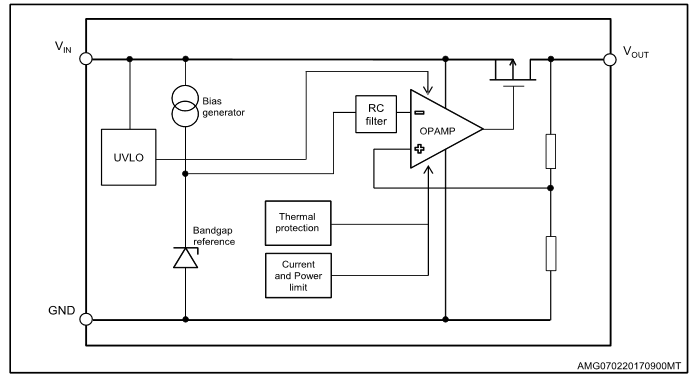
\includegraphics[width=350pt]{./Bilder/LDO.png}
	\caption{Blockschaltbild LDO}
	\label{fig:LDO}
\end{figure}

Der Differenzverstärker vergleicht die Ausgangsspannung mit einer stabilen Referenzquelle aus einer Zenerdiode, sodass diese gemessene Spannungsabweichung über das Stellglied ausgeregelt werden kann. Ist die Ausgangsspannung zu niedrig, so wird der Transistor stärker angesteuert bis die geforderte Ausgangsspannung erreicht wird, im umgekehrten Fall wird der Strom über den Transistor reduziert. Der Transistor wird in dieser Schaltung also quasi wie ein veränderlicher Widerstand verwendet, an dem die überflüssige Spannungsdifferenz abfällt und in Wärme umgewandelt wird. Die verwendeten LDOs besitzen außerdem eine Strombegrenzungsschaltung und eine Schutzschaltung, die die Betriebstemperatur überwacht und das Bauteil vor thermischer Überlastung schützt, sowie eine Unterspannungsabschaltung. 

\subsubsection{Verschaltung auf Platine}
Grund für die Wahl dieser Art von Spannungsreglern ist ihre kompakte Bauform, ihr günstiger Einkaufspreis und das geringe Rauschen im Vergleich zu Schaltreglern da keine Schaltvorgänge auftreten. Auf der Platine werden LDOs vom Typ LDL1117 von STMicroelectronics verwendet. Für die \SI{3,3}{V} Versorgung ist dies der LDL1117S33R und für die \SI{5}{V} der LDL1117S50R LDO. Nach dem Datenblatt \cite[S.7]{ldo} ist die Eingangskapazität zu \SI{1}{\mu F} und die Ausgangskapazität zu \SI{4,7}{\mu F} zu wählen. Diese werden aus Stabilitätsgründen und zur Entkopplung verwendet. Empfohlen wird weiterhin Keramikkondensatoren zu verwenden, welche X5R oder X7R Dielektrika aufweisen. In \autoref{fig:volt} ist der Schaltplan der Spannungsversorgung für die Platine zu sehen. An VIN wird die Batteriespannung angelegt, welche mit \SI{1}{\mu F} gegen GND entkoppelt wird. An VOUT liegen die jeweiligen \SI{3,3}{V} bzw. \SI{5}{V} an, welche jeweils über \SI{4,7}{\mu F} gegen GND geschaltet sind. Zur allgemeinen Spannungsglättung wird eine große Kapazität zwischen der Batteriespannung und GND geschaltet, welche starke Schwankungen beim Durchschalten der H-Brücke verhindern soll.

\begin{figure}[H]%
\centering
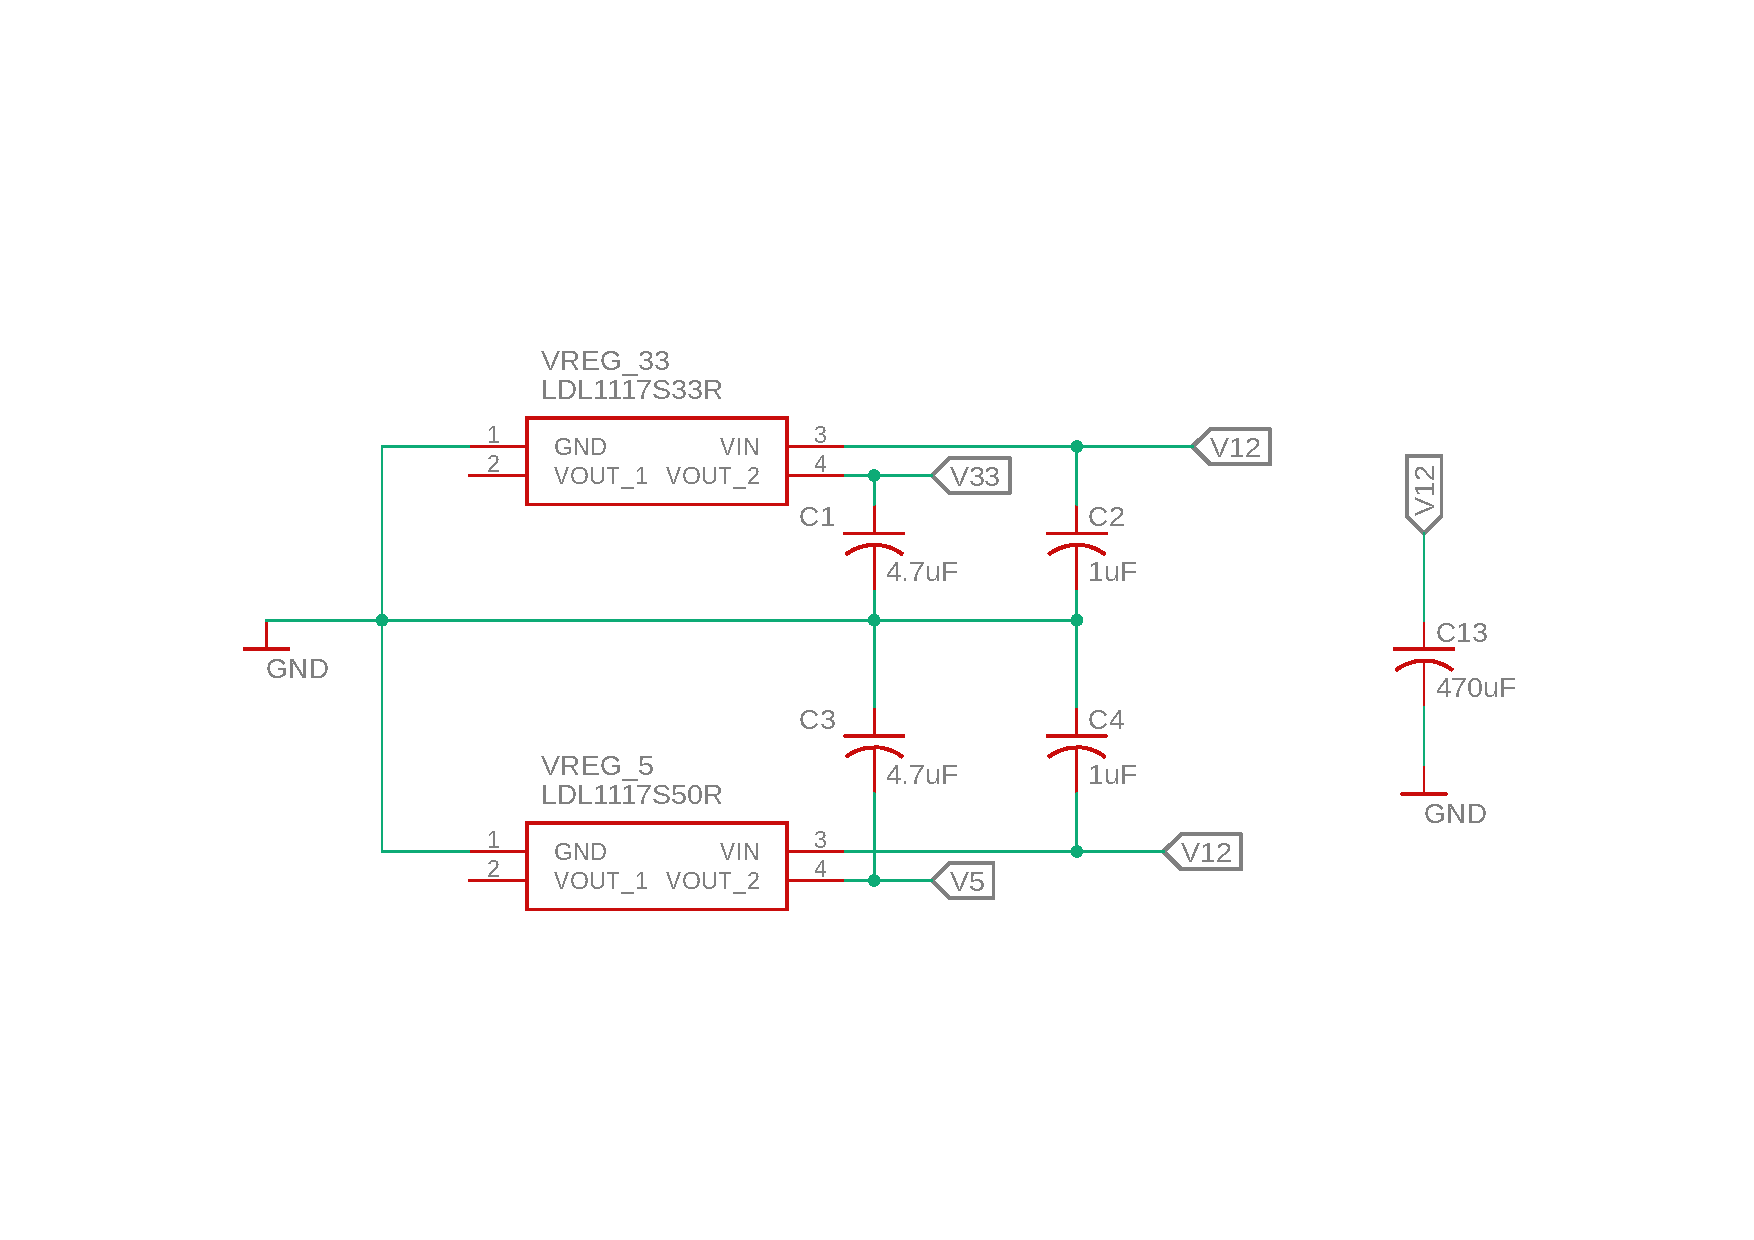
\includegraphics[width=400pt]{./Bilder/volt.pdf}%
\caption{Schaltplan Spannungsversorgung}%
\label{fig:volt}%
\end{figure}

\section{Platinenanschluss}
Die Platine wird mit einem 1-776267-1 von TE Connectivity verbunden um notwendige Signalleitungen nach außen zu führen und zusätzlich Spannungsversorgung und Lagesensorik mit der Platine verbinden zu können. In \autoref{fig:stecker} ist die Pin-Belegung des Steckers zu sehen. Um den Mikrocontroller über SWD programmieren zu können, muss der Stecker die notwendigen Signalleitungen SWDIO, SWCLK, TRACESWO, V33 und GND nach außen führen. Über diese Pins können über einen ST-Link/V2 Programme von einem Computer auf den Mikrocontroller übertragen werden. Weiterhin soll der Mikrocontroller über CAN-Signale mit der MicroAutobox kommunizieren können. Dazu werden die Schnittstellen CANH(CAN-HIGH) und CANL(CAN-LOW) über den Stecker nach außen geführt. Die Steckerpins V5, L\_1, L\_2 und GND werden für die Lagesensorik benötigt. Pin 4 und Pin 5 sind beide mit der Batterie verbunden und bilden die Spannungsversorgung der gesamten Platine. Aufgrund der potentiell hohen Ströme wird die Versorgung über zwei Pins zugeführt. Über den NRST-Pin lässt sich der Mikrocontroller zurücksetzen.

\begin{figure}[H]%
\centering
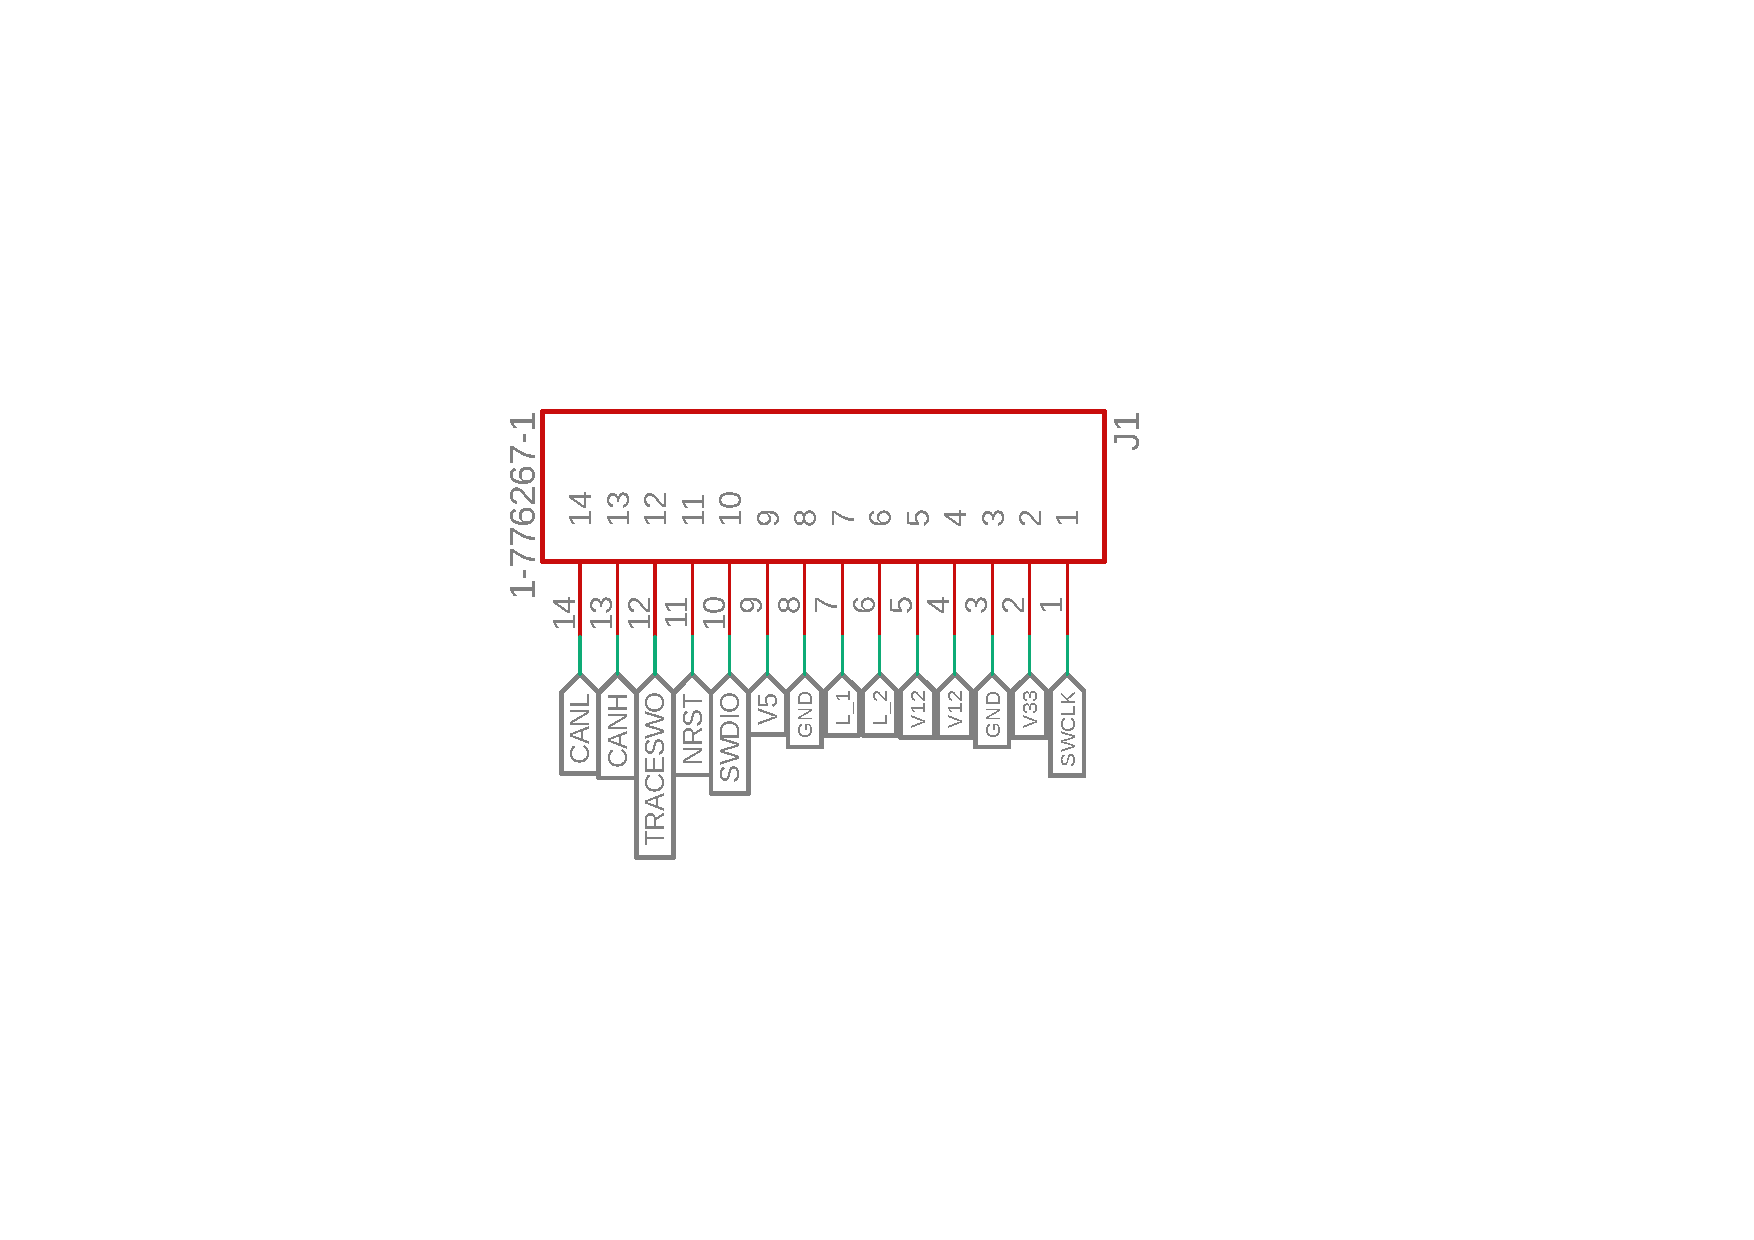
\includegraphics[width=200pt]{./Bilder/stecker.pdf}%
\caption{Anschlusspins Stecker}%
\label{fig:stecker}%
\end{figure}

\section{H-Brücke}
Jonas fragen.

\section{Sensorik}
Malte fragen.
